\documentclass[border=8pt]{standalone}
\usepackage[T1]{fontenc}
\usepackage{lmodern}
\usepackage{tikz}
\usetikzlibrary{positioning, fit, arrows.meta, calc}

% NYU brand colors
\definecolor{Navy}    {HTML}{330662}
\definecolor{Blue}    {HTML}{57068c}
\definecolor{UltraV}  {HTML}{8900e1}
\definecolor{LightBlu}{HTML}{eee6f3}
\definecolor{SlateGry}{HTML}{6d6d6d}
\definecolor{OffWhite}{HTML}{f2f2f2}
\definecolor{GoodGrn} {HTML}{009b8a}
\definecolor{AccentYl}{HTML}{59B2D1}

\begin{document}
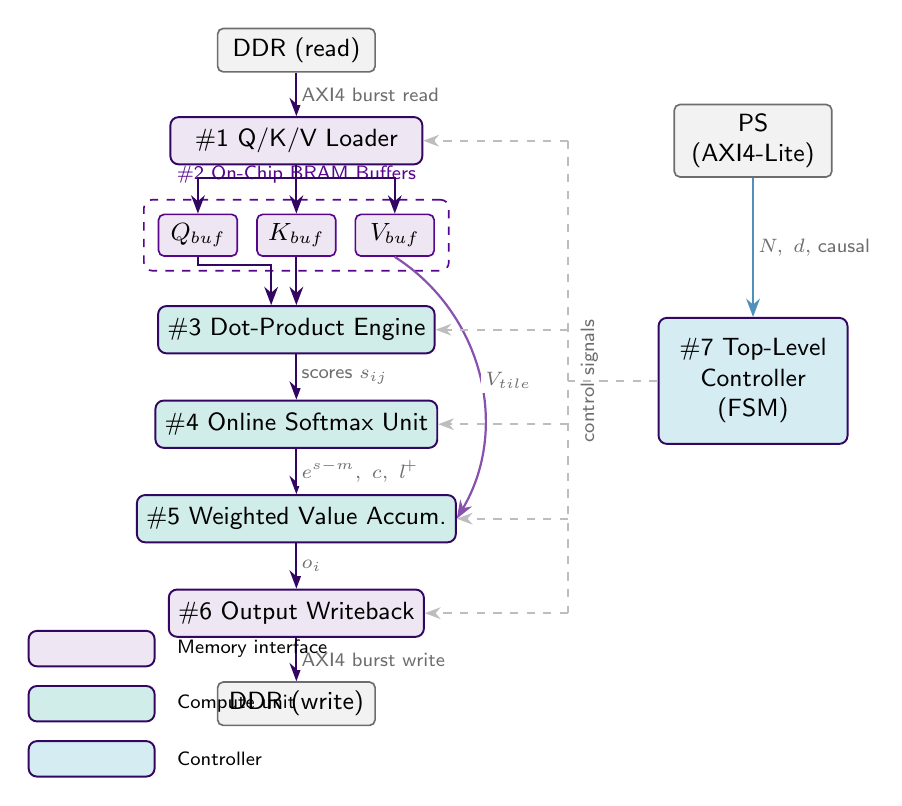
\begin{tikzpicture}[
  font=\small\sffamily, >=Stealth,
  every node/.style={align=center},
  mem/.style    = {draw=Navy, fill=LightBlu, rounded corners=3pt,
                   minimum width=3.2cm, minimum height=0.60cm, line width=0.7pt},
  compute/.style= {draw=Navy, fill=GoodGrn!18, rounded corners=3pt,
                   minimum width=3.2cm, minimum height=0.60cm, line width=0.7pt},
  ext/.style    = {draw=SlateGry, fill=OffWhite, rounded corners=2pt,
                   minimum width=2.0cm, minimum height=0.55cm, line width=0.6pt},
  ctrl/.style   = {draw=Navy, fill=AccentYl!25, rounded corners=3pt,
                   minimum width=2.4cm, minimum height=1.6cm, line width=0.7pt},
  buf/.style    = {draw=Blue, fill=LightBlu, rounded corners=2pt,
                   minimum width=1.0cm, minimum height=0.52cm, line width=0.6pt},
  sig/.style    = {font=\scriptsize\sffamily, fill=white, inner sep=1.5pt,
                   text=SlateGry},
]

% ── Main pipeline ─────────────────────────────────────────────────────────────
\node[ext]     (ddr_r) at (0,   0   ) {DDR (read)};
\node[mem]     (loader)at (0,  -1.15) {\#1\ Q/K/V Loader};

\node[buf]     (qbuf)  at (-1.25,-2.35) {$Q_{buf}$};
\node[buf]     (kbuf)  at (   0, -2.35) {$K_{buf}$};
\node[buf]     (vbuf)  at ( 1.25,-2.35) {$V_{buf}$};
\node[draw=Blue, dashed, rounded corners=3pt, inner sep=5pt, line width=0.6pt,
      fit=(qbuf)(kbuf)(vbuf),
      label={[font=\scriptsize\sffamily, text=Blue, yshift=2pt]above:\#2\ On-Chip BRAM Buffers}]{};

\node[compute] (dp)    at (0,  -3.55) {\#3\ Dot-Product Engine};
\node[compute] (sfx)   at (0,  -4.75) {\#4\ Online Softmax Unit};
\node[compute] (acc)   at (0,  -5.95) {\#5\ Weighted Value Accum.};
\node[mem]     (wb)    at (0,  -7.15) {\#6\ Output Writeback};
\node[ext]     (ddr_w) at (0,  -8.30) {DDR (write)};

% ── Controller / PS ───────────────────────────────────────────────────────────
\node[ext]  (ps)  at (5.8, -1.15) {PS\\(AXI4-Lite)};
\node[ctrl] (ctl) at (5.8, -4.20) {\#7\ Top-Level\\Controller\\(FSM)};

% ── Data arrows ───────────────────────────────────────────────────────────────
\draw[->, line width=0.8pt, Navy]
  (ddr_r) -- node[sig, right]{AXI4 burst read} (loader);

\draw[->, line width=0.8pt, Navy]
  (loader.south) -- ++(0,-0.16) -| (qbuf.north);
\draw[->, line width=0.8pt, Navy]
  (loader.south) -- ++(0,-0.16) -- (kbuf.north);
\draw[->, line width=0.8pt, Navy]
  (loader.south) -- ++(0,-0.16) -| (vbuf.north);

\draw[->, line width=0.8pt, Navy]
  (qbuf.south) -- ++(0,-0.10) -| ([xshift=-0.32cm]dp.north);
\draw[->, line width=0.8pt, Navy]
  (kbuf.south) -- (dp.north);

\draw[->, bend left=44, line width=0.8pt, Blue!70]
  (vbuf.south) to node[sig, pos=0.52, right]{$V_{tile}$} (acc.east);

\draw[->, line width=0.8pt, Navy]
  (dp)  -- node[sig, right]{scores $s_{ij}$}           (sfx);
\draw[->, line width=0.8pt, Navy]
  (sfx) -- node[sig, right]{$e^{s-m},\ c,\ l^{\!+}$}  (acc);
\draw[->, line width=0.8pt, Navy]
  (acc) -- node[sig, right]{$o_i$}                     (wb);
\draw[->, line width=0.8pt, Navy]
  (wb)  -- node[sig, right]{AXI4 burst write}           (ddr_w);

% ── PS → controller ───────────────────────────────────────────────────────────
\draw[->, line width=0.8pt, AccentYl!80!Navy]
  (ps) -- node[sig, right]{$N,\;d,\;$causal} (ctl);

% ── Control bus ───────────────────────────────────────────────────────────────
\coordinate (bt) at (3.45,-1.15);
\coordinate (bb) at (3.45,-7.15);
\draw[SlateGry!45, dashed, line width=0.6pt] (ctl.west) -- (3.45,-4.20);
\draw[SlateGry!45, dashed, line width=0.6pt] (bt) -- (bb);
\foreach \y/\m in {-1.15/loader,-3.55/dp,-4.75/sfx,-5.95/acc,-7.15/wb}{
  \draw[->, SlateGry!45, dashed, line width=0.6pt] (3.45,\y) -- (\m.east);
}
\node[rotate=90, font=\scriptsize\sffamily, text=SlateGry]
  at (3.72,-4.20) {control signals};

% ── Legend ────────────────────────────────────────────────────────────────────
\node[mem,     minimum width=1.6cm, minimum height=0.45cm]
  (lm) at (-2.6,-7.6) {};
\node[compute, minimum width=1.6cm, minimum height=0.45cm]
  (lc) at (-2.6,-8.3) {};
\node[ctrl,    minimum width=1.6cm, minimum height=0.45cm]
  (lk) at (-2.6,-9.0) {};
\node[font=\scriptsize\sffamily, right=0.15cm of lm] {Memory interface};
\node[font=\scriptsize\sffamily, right=0.15cm of lc] {Compute unit};
\node[font=\scriptsize\sffamily, right=0.15cm of lk] {Controller};

\end{tikzpicture}
\end{document}
